\documentclass{article}
\usepackage[utf8]{inputenc}
\usepackage{url}
\usepackage{graphicx}
\usepackage{hyperref}
\usepackage{amsmath}
\graphicspath{ {./} }


\title{Automatisation du prétraitement de photographies de portraits de mandrills}
\author{Maxime Boucher}
\date{Compte rendu 8}

\begin{document}

\maketitle

Avec Claudia nous nous demandions si un remplacement du fichier CSV actuel par une base de données de type SQL ne permettrait pas un usage simplifié, notamment sur le partage de métadonnées entre photos de portraits, photos originales, et autres CSV sur lesquelles nous nous appuyons pour notamment la date de naissance.

Alors j'ai créé une base de données SQLite, sans serveur donc (ou file-based) pour profiter d'un moteur SQL tout en ayant aucun serveur à gérer (une sorte de fichier CSV donc mais plus organisé et utilisable).

\begin{center}
    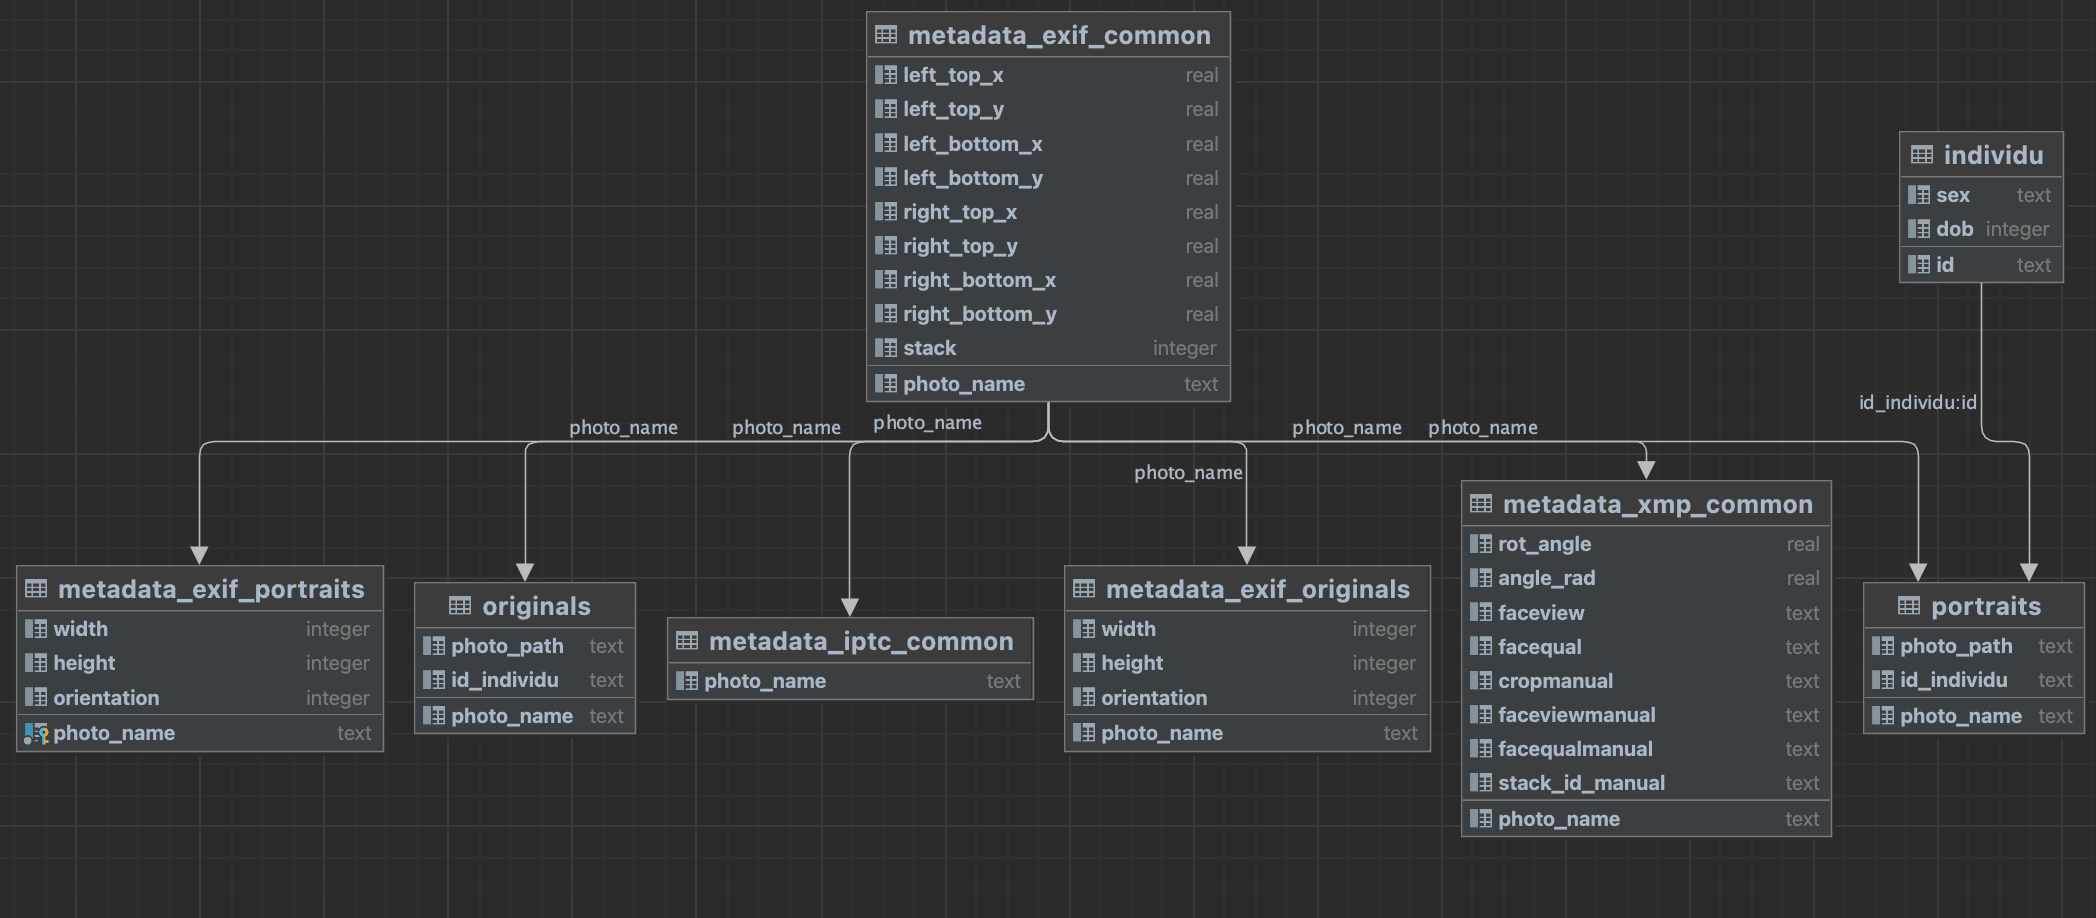
\includegraphics[width=345]{imgs/qualité/cr8/sqlite_schema.png}
\end{center}

J'ai par ailleurs calculé l'âge des mandrills en jours en faisant la formule suivante :
\begin{equation}
    age = date_{photo} - date_{naissance}
\end{equation}
\begin{center}
    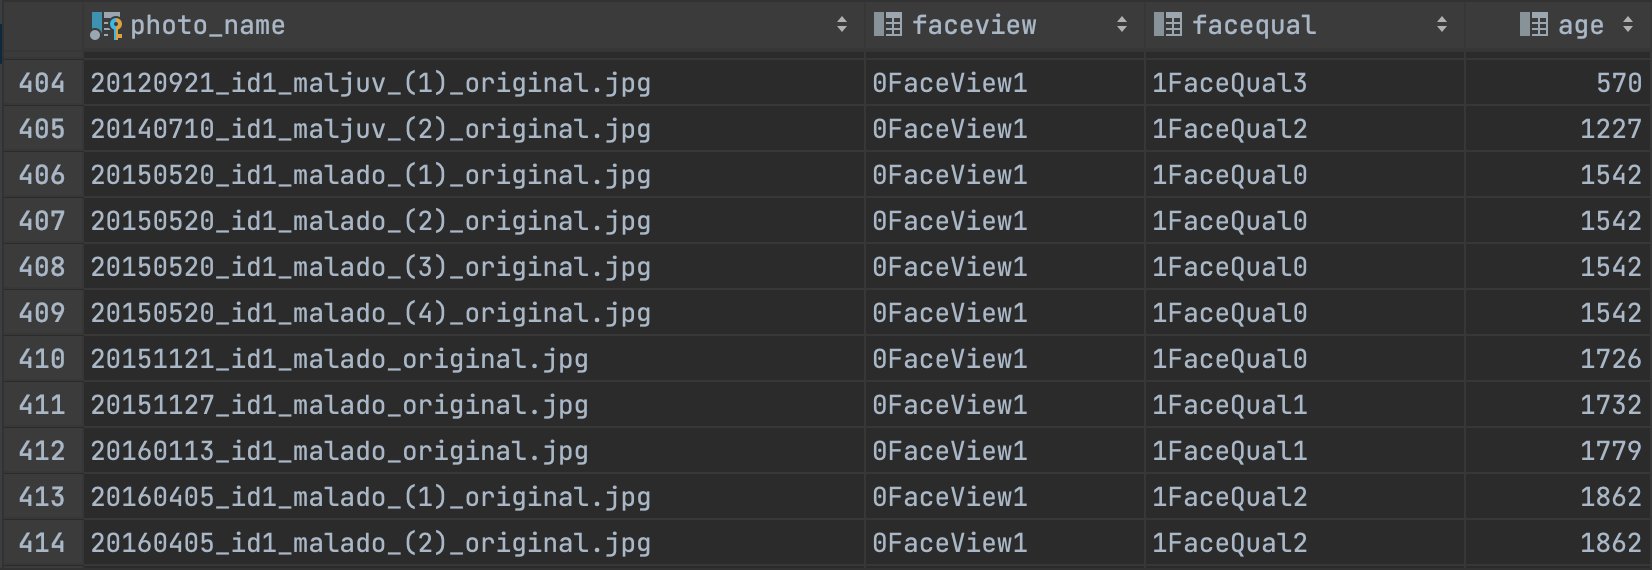
\includegraphics[width=345]{imgs/qualité/cr8/sql_query.png}
\end{center}

J'ai également essayé d'amélioré les résultats par rapport à la dernière fois, en dégelant toutes les couches de EfficientNet lors d'un 3e apprentissage, modifiant le drop out et la batch normalization, sans grand succès.\\
Pour ce qui est des images FaceQual0 générés à partir des images FaceQual0, le code est en place mais j'ai un doute sur le protocole d'utilisation des images. Actuellement, je charge le dataset initial, que je coupe en trois parties : train/validation/test. Ensuite, j'additionne le jeu d'entraînement avec les images générés, que je mélange de manière aléatoire.\\

Enfin, je vais continuer de travailler sur le débruitage des labels. Je travaille également sur l'utilisation de Docker pour que les environnements de travails soient mieux partagés (dans certains cas, Anaconda (ou miniconda) ne peut pas faire assez).

\end{document}
